\section{An ordinary hypergraph product}
\label{sec:hgp}

The construction below follows the ordinary hypergraph-product setting
of Tillich and Zemor~\cite{TillichZemor2009}. The small parameters later
in this section are an illustrative source claim, not a quoted table
from that paper.

\begin{thm}[Commutation of the block construction]
\label{thm:hgp-css}
\uses{def:css}
Let $H_1\in\mathbb{F}_2^{m_1\times n_1}$ and
$H_2\in\mathbb{F}_2^{m_2\times n_2}$. Define
\begin{align}
\label{eq:hgp-checks}
H_X&=[H_1\otimes I_{n_2}\mid I_{m_1}\otimes H_2^T],\\
H_Z&=[I_{n_1}\otimes H_2\mid H_1^T\otimes I_{m_2}].
\end{align}
Then $H_XH_Z^T=0$ over $\mathbb{F}_2$.
\end{thm}

\begin{proof}
\label{proof:hgp-css}
\uses{def:gf2,lem:css-commutation}
Multiplying the two blocks gives
\begin{equation}
\label{eq:hgp-commutation}
H_XH_Z^T=H_1\otimes H_2^T+H_1\otimes H_2^T=0.
\end{equation}
The last equality uses the field in Definition~\ref{def:gf2}.
Lemma~\ref{lem:css-commutation} identifies this binary identity with
pairwise commutation of the CSS generators.
\end{proof}

\begin{thm}[Length of the repetition-seed instance]
\label{thm:hgp-length}
Use the construction of Theorem~\ref{thm:hgp-css} with
\begin{equation}
\label{eq:repetition-seed}
H_1=H_2=
\begin{pmatrix}
1&1&0\\
0&1&1
\end{pmatrix}.
\end{equation}
The resulting presentation has thirteen data qubits.
\end{thm}

For background and motivation, compare Theorem~\ref{thm:hgp-css}.
This reference records a discussion link and is not a declaration
that the following table depends on a proof of that theorem.

\begin{table}[ht]
\centering
\caption{Intended finite-instance values in this source fixture.
The importer does not verify these parameters.}
\label{tab:rep3}
\begin{tabular}{lccc}
Construction & $n$ & $k$ & $d$\\
Ordinary HGP of two repetition seeds & 13 & 1 & 3
\end{tabular}
\end{table}

\begin{figure}[ht]
\centering
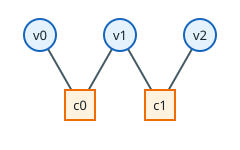
\includegraphics[width=0.6\linewidth]{figures/tanner-placeholder.svg}
\caption{The two-check graph of one length-three repetition seed.
This is not the full thirteen-qubit HGP graph.}
\label{fig:repetition-seed}
\end{figure}

% The proof is intentionally separated from its theorem by prose and floats.
\begin{proof}[Proof of Theorem~\ref{thm:hgp-length}]
\label{proof:hgp-length}
\proves{thm:hgp-length}
\uses{thm:hgp-css}
Each seed in Equation~\eqref{eq:repetition-seed} has $n_i=3$ columns
and $m_i=2$ rows. The first block in
Equation~\eqref{eq:hgp-checks} has $n_1n_2=9$ columns, and the second
has $m_1m_2=4$ columns. Hence $n=9+4=13$.
\end{proof}

\begin{example}[An explicit data claim]
\label{ex:rep3-parameters}
With column order $(i,j)\mapsto 3i+j$ for the first nine qubits and
$(a,b)\mapsto 9+2a+b$ for the remaining four qubits, the intended
instance is $[[13,1,3]]$. The rank and distance values can be checked
by binary linear algebra and exhaustive enumeration.
Table~\ref{tab:rep3} states those values, but this document does not
attach a computation report or a Lean certificate for them.
\end{example}
